\documentclass[aspectratio=169,11pt]{beamer}
\usetheme{default}
\setbeamertemplate{navigation symbols}{}
\setbeamertemplate{footline}{%
  \hfill\insertframenumber/\inserttotalframenumber\hspace*{4pt}\vspace{2pt}%
}
\usepackage{lmodern}
\usepackage[most]{tcolorbox}
\usepackage{listings}
\usepackage{tikz}
\usetikzlibrary{arrows.meta,positioning,shapes.geometric,fit,backgrounds}
\usepackage{booktabs}
\usepackage{hyperref}

\definecolor{lcgreen}{HTML}{2E7D32}
\definecolor{lcblue}{HTML}{1565C0}
\definecolor{lcorange}{HTML}{EF6C00}
\definecolor{lcred}{HTML}{C62828}
\definecolor{codebg}{HTML}{F5F5F5}
\definecolor{docgray}{gray}{0.55}

\newtcolorbox{conceptbox}[1][]{colback=yellow!20,colframe=yellow!60!black,title=#1,fonttitle=\bfseries,top=2pt,bottom=2pt,left=4pt,right=4pt}
\newtcolorbox{warningbox}[1][]{colback=red!15,colframe=red!60!black,title=#1,fonttitle=\bfseries,top=2pt,bottom=2pt,left=4pt,right=4pt}
\newtcolorbox{tipbox}[1][]{colback=green!10,colframe=green!50!black,title=#1,fonttitle=\bfseries,top=2pt,bottom=2pt,left=4pt,right=4pt}
\newtcolorbox{codebox}[1][]{colback=blue!10,colframe=blue!40!black,title=#1,fonttitle=\bfseries,top=2pt,bottom=2pt,left=4pt,right=4pt}

\lstset{
  basicstyle=\ttfamily\scriptsize,
  backgroundcolor=\color{codebg},
  breaklines=true,
  frame=single,
  rulecolor=\color{blue!40!black},
  keywordstyle=\color{lcblue}\bfseries,
  stringstyle=\color{lcgreen},
  commentstyle=\color{docgray}\itshape,
  language=Python,
  showstringspaces=false,
  tabsize=2,
  xleftmargin=2pt,
  xrightmargin=2pt,
  aboveskip=2pt,
  belowskip=2pt,
}

\newcommand{\docref}[1]{{\scriptsize\color{docgray}[Docs: #1]}}

\title{Section 05: Prebuilt ReAct Agent}
\subtitle{The Reason + Act Pattern as a Graph}
\author{LangGraph v1.0.x (March 2026)}
\date{}

\begin{document}

\frame{\titlepage}

\begin{frame}{Mental Model: ReAct Pattern}
  \begin{conceptbox}[The Big Picture]
    \setlength{\itemsep}{1pt}
    \begin{itemize}
      \item \textbf{ReAct}: Reason + Act (Yao et al., 2023)
      \item Agent \textbf{thinks} about a problem, \textbf{acts} via tools, \textbf{observes} results
      \item Loop: Think -> Act → Observe → Think → \ldots
      \item Much more effective than just chain-of-thought
    \end{itemize}
  \end{conceptbox}
  \vspace{0.1cm}
  \begin{tipbox}[Why It Works]
    Grounding reasoning in real-world interaction beats pure reasoning.
  \end{tipbox}
\end{frame}

\begin{frame}{What Is ReAct: The Loop}
  \begin{conceptbox}[ReAct Cycle]
    \setlength{\itemsep}{1pt}
    \begin{itemize}
      \item \textbf{Observe}: Read the problem and current context
      \item \textbf{Think}: Reason about what to do next
      \item \textbf{Act}: Call a tool to gather information or take action
      \item \textbf{Observe}: See the result, decide to continue or stop
      \item \textbf{Repeat} until goal is reached or max steps exceeded
    \end{itemize}
  \end{conceptbox}
  \vspace{0.1cm}
  \begin{tipbox}[Key Advantage]
    Can recover from mistakes: if a tool call fails, agent \textbf{reasons} about the failure.
  \end{tipbox}
\end{frame}

\begin{frame}[fragile]{create\_react\_agent: The High-Level Shortcut}
  \begin{codebox}[Basic Usage]
    \begin{lstlisting}
from langgraph.prebuilt import create_react_agent
from langchain_openai import ChatOpenAI
model = ChatOpenAI(model="gpt-4")
tools = [get_weather, search_docs, add_numbers]
agent = create_react_agent(model, tools)
result = agent.invoke({
  "messages": [HumanMessage("What's the weather?")]
})
print(result["messages"][-1].content)
    \end{lstlisting}
  \end{codebox}
  \vspace{0.1cm}
  \begin{tipbox}[One-Liner Magic]
    \texttt{create\_react\_agent()} builds a complete agent in seconds.
  \end{tipbox}
\end{frame}

\begin{frame}[fragile,shrink=5]{What create\_react\_agent Builds Under the Hood}
  \begin{codebox}[Equivalent Manual Graph]
    \begin{lstlisting}
builder = StateGraph(MessagesState)
builder.add_node("agent", lambda state: {
  "messages": [model.invoke(state["messages"])]
})
builder.add_node("tools", ToolNode(tools))
builder.add_edge(START, "agent")
builder.add_conditional_edges(
  "agent", tools_condition,
  {"tools": "tools", END: END}
)
builder.add_edge("tools", "agent")
graph = builder.compile()
    \end{lstlisting}
  \end{codebox}
  \begin{tipbox}[Demystified]
    \texttt{create\_react\_agent} is just StateGraph + ToolNode + tools\_condition.
  \end{tipbox}
\end{frame}

\begin{frame}{TikZ Diagram: ReAct Agent Graph Structure}
  \begin{center}
    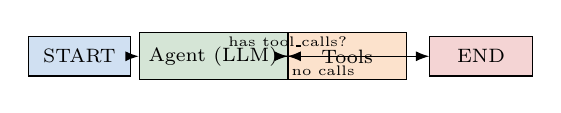
\begin{tikzpicture}[scale=0.85, every node/.style={font=\scriptsize}]
      \node[draw, rectangle, fill=lcblue!20, minimum width=1.3cm, minimum height=0.5cm] (start) at (0, 2) {START};
      \node[draw, rectangle, fill=lcgreen!20, minimum width=1.5cm, minimum height=0.6cm] (agent) at (2, 2) {Agent (LLM)};
      \node[draw, rectangle, fill=lcorange!20, minimum width=1.5cm, minimum height=0.6cm] (tools) at (4, 2) {Tools};
      \node[draw, rectangle, fill=lcred!20, minimum width=1.3cm, minimum height=0.5cm] (end) at (6, 2) {END};
      \draw[-Latex] (start) -- (agent);
      \draw[-Latex] (agent) -- node[above]{\tiny has tool\_calls?} (tools);
      \draw[-Latex] (agent) -- node[below,near start]{\tiny no calls} (end);
      \draw[-Latex, bend right] (tools) -- (agent);
    \end{tikzpicture}
  \end{center}
  \vspace{0.1cm}
  \begin{tipbox}[Agent Loop]
    Tools flow back to Agent. Loop continues until agent stops calling tools.
  \end{tipbox}
\end{frame}

\begin{frame}[fragile]{Customizing the System Prompt}
  \begin{codebox}[Custom Prompt Example]
    \begin{lstlisting}
from langchain_core.prompts import ChatPromptTemplate
system_prompt = """You are a helpful AI assistant.
Always be concise. Use tools when needed."""
prompt = ChatPromptTemplate.from_messages([
  ("system", system_prompt),
  ("placeholder", "{messages}")
])
agent = create_react_agent(
  model,
  tools,
  prompt=prompt
)
    \end{lstlisting}
  \end{codebox}
  \vspace{0.1cm}
  \begin{tipbox}[Prompt Matters]
    System prompt shapes agent behavior. Experiment with tone, constraints, guidelines.
  \end{tipbox}
\end{frame}

\begin{frame}[fragile]{Adding a Checkpointer for Persistence}
  \begin{codebox}[Persistence Setup]
    \begin{lstlisting}
from langgraph.checkpoint.memory import MemorySaver
checkpointer = MemorySaver()
agent = create_react_agent(
  model,
  tools,
  checkpointer=checkpointer
)
config = {"configurable": {"thread_id": "user_123"}}
result = agent.invoke(
  {"messages": [HumanMessage("Hi")]},
  config=config
)
    \end{lstlisting}
  \end{codebox}
  \vspace{0.1cm}
  \begin{tipbox}[Enables Resumption]
    Checkpointer + thread\_id allow conversations to persist across invocations.
  \end{tipbox}
\end{frame}

\begin{frame}[fragile]{Adding Message History and Memory}
  \begin{codebox}[History Pattern]
    \begin{lstlisting}
def load_messages_from_db(user_id):
  """Simulate loading from database."""
  return get_user_history(user_id)
config = {"configurable": {"thread_id": "user_123"}}
old_messages = agent.get_state(config)["messages"]
new_input = HumanMessage("Follow up question?")
result = agent.invoke(
  {"messages": old_messages + [new_input]},
  config=config
)
    \end{lstlisting}
  \end{codebox}
  \vspace{0.1cm}
  \begin{tipbox}[Stateful Agents]
    Checkpointer handles message history automatically if you \texttt{invoke} with config.
  \end{tipbox}
\end{frame}

\begin{frame}[fragile]{Customizing with state\_modifier}
  \begin{codebox}[state\_modifier Hook]
    \begin{lstlisting}
def modify_state(state):
  """Pre-process state before model invocation."""
  # Add context, filter messages, etc.
  if len(state["messages"]) > 10:
    state["messages"] = state["messages"][-10:]
  return state
agent = create_react_agent(
  model,
  tools,
  state_modifier=modify_state
)
    \end{lstlisting}
  \end{codebox}
  \vspace{0.1cm}
  \begin{tipbox}[Advanced Customization]
    state\_modifier lets you inject custom logic before model invocation.
  \end{tipbox}
\end{frame}

\begin{frame}[fragile]{Pre-processing and Post-processing Hooks}
  \begin{codebox}[Custom Hooks]
    \begin{lstlisting}
def log_invocation(state):
  print(f"Messages: {len(state['messages'])}")
  return state
def log_completion(state):
  print(f"Final message: {state['messages'][-1]}")
  return state
agent = create_react_agent(model, tools)
agent = agent.map_nodes(
  lambda node: (log_invocation >> node >> log_completion)
  if node.name == "agent" else node
)
    \end{lstlisting}
  \end{codebox}
  \vspace{0.1cm}
  \begin{tipbox}[Debugging and Observability]
    Hooks enable logging, monitoring, and state inspection.
  \end{tipbox}
\end{frame}

\begin{frame}{When to Use Prebuilt vs Custom Graph}
  \begin{conceptbox}[Use Prebuilt ReAct If]
    \setlength{\itemsep}{1pt}
    \begin{itemize}
      \item Simple reason-act loop is enough
      \item Standard tool calling, no custom nodes
      \item Want fast prototyping
    \end{itemize}
  \end{conceptbox}
  \vspace{0.1cm}
  \begin{warningbox}[Use Custom StateGraph If]
    \setlength{\itemsep}{1pt}
    \begin{itemize}
      \item Multiple agent teams or parallel branches
      \item Complex approval/human-in-the-loop workflows
      \item Custom node logic, state transformations
    \end{itemize}
  \end{warningbox}
\end{frame}

\begin{frame}[fragile]{Comparison: Prebuilt vs Custom}
  \begin{center}
    \footnotesize
    \begin{tabular}{|l|l|l|}
      \hline
      \textbf{Aspect} & \textbf{Prebuilt} & \textbf{Custom} \\
      \hline
      Lines of code & 5--10 & 50--200 \\
      \hline
      Setup time & Seconds & Minutes \\
      \hline
      Flexibility & Limited & Full \\
      \hline
      Debugging & Opaque & Transparent \\
      \hline
      Multiple agents & No & Yes \\
      \hline
      Human interrupts & Limited & Full \\
      \hline
    \end{tabular}
  \end{center}
  \vspace{0.15cm}
  \begin{tipbox}[Strategy]
    Start with prebuilt. Migrate to custom when you hit limitations.
  \end{tipbox}
\end{frame}

\begin{frame}{Limitations of the Prebuilt Agent}
  \begin{warningbox}[What You Can't Do]
    \setlength{\itemsep}{1pt}
    \begin{itemize}
      \item No parallel tool execution
      \item No inter-agent communication
      \item Limited human-in-the-loop control
      \item Can't easily add custom logic between nodes
      \item Fixed agent -> tools → agent loop
    \end{itemize}
  \end{warningbox}
  \vspace{0.1cm}
  \begin{tipbox}[When to Outgrow]
    Once you need more than reason + act, build a custom graph.
  \end{tipbox}
\end{frame}

\begin{frame}[fragile]{Migrating from Prebuilt to Custom}
  \begin{codebox}[Refactor Pattern]
    \begin{lstlisting}
# Was using prebuilt
agent = create_react_agent(model, tools)
# Now building custom
from langgraph.graph import StateGraph, START, END
builder = StateGraph(MessagesState)
builder.add_node("agent", agent_node)
builder.add_node("tools", ToolNode(tools))
builder.add_edge(START, "agent")
builder.add_conditional_edges(
  "agent", tools_condition, ...
)
custom_agent = builder.compile(...)
    \end{lstlisting}
  \end{codebox}
  \vspace{0.1cm}
  \begin{tipbox}[Smooth Transition]
    Extract prebuilt logic and customize node by node.
  \end{tipbox}
\end{frame}

\begin{frame}[fragile]{Summary: ReAct Cheat Sheet}
  \begin{codebox}[Quick Start]
    \begin{lstlisting}
from langgraph.prebuilt import create_react_agent
agent = create_react_agent(
  ChatOpenAI(model="gpt-4"),
  [tool1, tool2, ...]
)
result = agent.invoke({
  "messages": [HumanMessage("Task")]
})
print(result["messages"][-1])
    \end{lstlisting}
  \end{codebox}
  \vspace{0.1cm}
  \begin{tipbox}[Remember]
    Prebuilt ReAct is fast, but custom graphs are powerful. Pick the right tool.
  \end{tipbox}
\end{frame}

\begin{frame}{Self-Check: Do You Understand?}
  \begin{enumerate}
    \setlength{\itemsep}{1pt}
    \item What does ReAct stand for and why is it effective?
    \item How many lines of code are in a minimal \texttt{create\_react\_agent} call?
    \item What does \texttt{state\_modifier} let you do?
    \item When should you build a custom graph instead of using prebuilt?
    \item How does persistence (checkpointer) change agent behavior?
    \item What's the difference between Prebuilt and StateGraph approaches?
    \item How do you add custom logic to a prebuilt agent?
  \end{enumerate}
\end{frame}

\end{document}
